In the context of this project, accessibility refers to considerations for users with visual, auditory, cognitive and/or physical impairments; inclusiveness refers to considerations for users for whom English isn't their first language, older users and users with gender or affective issues; and universal design refers to compatibility of Magpie with different devices, browsers and networks.\\

\noindent The accessibility general guidelines we'll be evaluating Magpie on are from the EU Web Accessibility Directive which directly affect public bodies in Ireland although map systems are exempt. This directive came into effect at the end of 2016 and aims to \emph{make public sector websites and mobile applications more accessible, and to harmonise varying standards within the European Union (\ldots)} (\cite{webaccessibilitydirective2016}).\\
%figure for accessibility guidelines
\begin{figure}[h!]
    \centering
    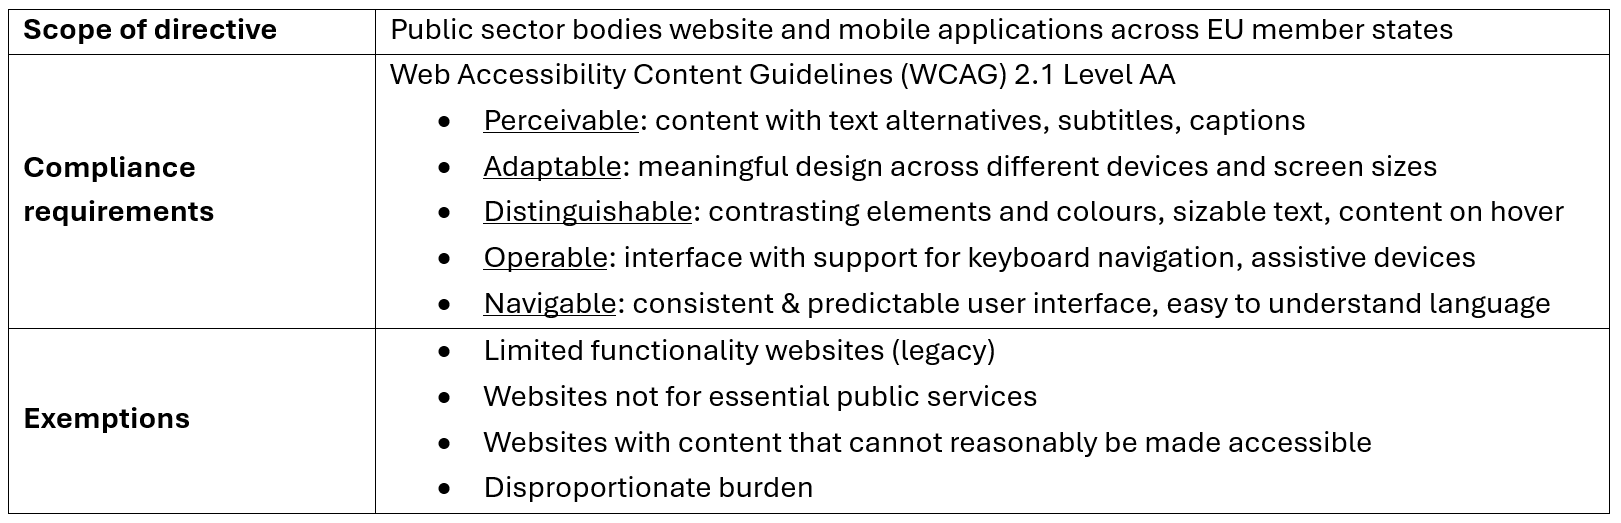
\includegraphics[width=0.85\textwidth]{images/wcag-guidelines.png}
    \caption{WCAG 2.1 Scope, Guidelines \& Exemptions}
\end{figure}

\noindent There is an inherent limitation of accessibility for map\-based systems due to their visual nature.\\
Visual impairment is categorized as having a type of eye disorder and/or a degree of vision loss; an estimate of 2.2 billion people globally have vision impairment (\cite{whoworldreportvision2019}) and 297,000 (5.6\%) of the population in Ireland(\cite{visionirelandcensus}).\\

\noindent The paper by \cite{accessibilitywebmapsrecommendations2017} which relied on data from two projects aimed at developing web\-map applications for visually impaired individuals has presented several recommendations, the following which we will guide Magpie's accessibility evaluation and subsequent iterative development:
\begin{itemize}
    \item\textbf{UI components:} Creating a UI that is simple, understandable and follows a clear predictable layout. Implement only necessary control elements, group them by similar focus and place them in areas that are familiar (similar in other programs). The UI should be flat while avoiding dropdowns, scrolling and nested/overlapping elements. Control elements overlapping the map makes it difficult for visually impaired users to read the map and use the controls, so this practice should be avoided.\\
    \item\textbf{UI design:} Size and colour of UI components should be chosen to provide high contrast between different elements; if symbols are used they should be easily recognizable and complex backgrounds should be avoided.\\
    \item\textbf{UI language:} Familiar and easy recognizable terms should be used on the interface so as to not scare off users with unknown technical terms and make the application accessible to all.\\
    \item\textbf{UI interaction:} A user should be able to interact with the interface using both a mouse and keyboard on desktop; keyboard accessibility is key for improving accessibility for visually impaired users.
\end{itemize}

\newpage
\noindent We requested a review from Accessibility expert Damian Gordon.\\
He served on the board of the National Disability Authority, who advise the Irish Government on all matters related to disability, and he has worked with a wide range of disability organisations, include the Centre Remedial Clinic, the National Council for the Blind, Arthritis Ireland, and the Aging\-Well Network. He has contributed to the development of hardware, software, legislation and training related to disability awareness and accessibility. \\

\noindent The goal of this review is to evaluate the accessibility, inclusivity \& universal design of Magpie with regards to the guidelines and recommendations detailed above.\\

\noindent The review was conducted on November 21st during the usability testing phase of Magpie. The session was conducted online through videoconference meeting on Teams where we presented Magpie, gave Damian Gordon a scenario to follow to explore the application, discuss the scenario and the accessibility guidelines and then a survey.\\\\
The scenario given can be seen in the table below. A scenario was given so as to simulate the use of Magpie by one of our target users through the lens of an accessibility expert.\\
%table for scenario
\begin{table}[h!]
    \centering
    \caption{Scenario for the Accessibility review}
    \begin{tabular}{|p{0.9\textwidth}|}
        \hline
        \textbf{Scenario:}                                                                                                                                                                                                                                                                                         \\
        \hline
        You are an architect contracted by Dublin City Council to expand the Dominick Street Recreation Centre, located on Dominick Street Lower, Dublin 1. As part of your assignment, you need to plan the expansion in a way that integrates effectively with the surrounding community and existing amenities. \\
        \hline
        \textbf{Scenario tasks:}                                                                                                                                                                                                                                                                                   \\
        \hline
        \begin{enumerate}
            \item \textbf{Locate the Community Centre:} Use the GIS application to locate the Dominick Street Recreation Centre on the map.
            \item \textbf{Identify nearby amenities:} Select the public amenities you think are relevant within a 500-meter radius of the recreation centre. These can include but are not limited to: bicycle stands, parking spaces, public wi-fi spots, public toilets.
            \item \textbf{Analyse amenity density:} Based on your findings, determine which types of amenities are abundant and which are lacking around the centre.
            \item \textbf{Assess accesibility:} Check how accessible the recreation centre is by identifying nearby transportation options. Note any gaps in accessibility that might need addressing.
            \item \textbf{Plan for additional amenities:} Suggest which new amenities should be added as part of the recreation centre's expansion to better serve the community. For example: if car parking is insufficient, recommend additional parking spaces.
        \end{enumerate}                                              \\
        \hline
    \end{tabular}
\end{table}

\noindent The questionnaire covers UI design, interaction and language and aims to complement the vocal feedback of the session. It is made up of 3 sections with a mixture of closed questions rating different parts of the system, and open questions to provide more qualitative feedback.\\

\noindent We are also observing Damian Gordon's behaviour and if he was able to complete general tasks related to the main features of Magpie. The results can be seen in the table below, it recorded if they were able to complete the task, how difficult it was for them based on behavioural cues and any errors bugs encountered during the task. We were not able to record the time taken for each task due to the informal administration of them, the user was not aware we were 'grading' them in a sense.\\

\noindent The difficulty of the task is related to if they were able to complete it and how much they struggled during it. The status of a task can either be `complete', `pass' or `fail' where `complete' is attributed when the user does the task on their own, `pass' is attributed when the user was able to complete the task but with our help, and `fail' when the user were not able to do the task even with our help. \\
%table for general tasks completion & difficulty
\begin{table}[h!]
    \centering
    \caption{General tasks score for the Accessibility review}
    \begin{tabular}{|p{0.3\textwidth}|p{0.1\textwidth}|p{0.1\textwidth}|p{0.3\textwidth}|}
        \hline
        \textbf{General task:}           & \textbf{Status} & \textbf{Difficulty} & \textbf{Errors}                                                                   \\
        \hline
        Load Magpie application          & Complete        & 1                   &                                                                                   \\
        \hline
        Sign up new account              & Complete        & 1                   &                                                                                   \\
        \hline
        Log in                           & Complete        & 1                   &                                                                                   \\
        \hline
        Go through onboarding            & Pass            & 2                   & Technical issues with onboarding overlay + user tried to click on locked elements \\
        \hline
        Place cursor on map              & Complete        & 1                   &                                                                                   \\
        \hline
        Zoom in and out                  & Fail            & 5                   & Did not know how to use the mouse + onboarding confusing                          \\
        \hline
        Hold map and navigate            & Complete        & 2                   &                                                                                   \\
        \hline
        Adjust radius big/small          & Complete        & 1                   &                                                                                   \\
        \hline
        Clear marker and radius from map & N/A             & N/A                 & Feature not used                                                                  \\
        \hline
        Deselect all amenities           & Complete        & 1                   &                                                                                   \\
        \hline
        Choose certain amenities         & Complete        & 1                   &                                                                                   \\
        \hline
        Find onboarding and exit midway  & Pass            & 4                   & Could not find onboarding button                                                  \\
        \hline
        Logout                           & Pass            & 3                   & Could not find profile button                                                     \\
        \hline
    \end{tabular}
\end{table}

\newpage
\noindent The review provided some useful insights with regards to missing features to complete the scenario and areas of Magpie that comply with accessibility standards. Below were the main takeaways:\\\\
\textbf{Dashboard: }
Damian Gordon had some trouble locating the recreation centre during the scenario, and advise that have a search bar would remove the difficulty and give options for those who may be visually impaired to find a location on the map, and also for those who may not know where the area they're looking for is located.\\\\
\textbf{Onboarding: }
Damian Gordon found the steps in the onboarding very wordy and too long, which may cause some users to skip through or not retain the information present there. In addition, some of the wording could be improved related to navigating the map as shown in the figure below. This issue was further illustrated by the difficulty Damian Gordon encountered trying to zoom in and out on the map using his mousepad, having not understood how to do it from the onboarding step 5 that explain how to do it with a 'mouse' and a 'touchpad'. Addressing the choice of words, the content and flow of the onboarding is important to ensure it is understood by all kinds of users.\\
%figure for the old confusing onboarding
\begin{figure}[h!]
    \centering
    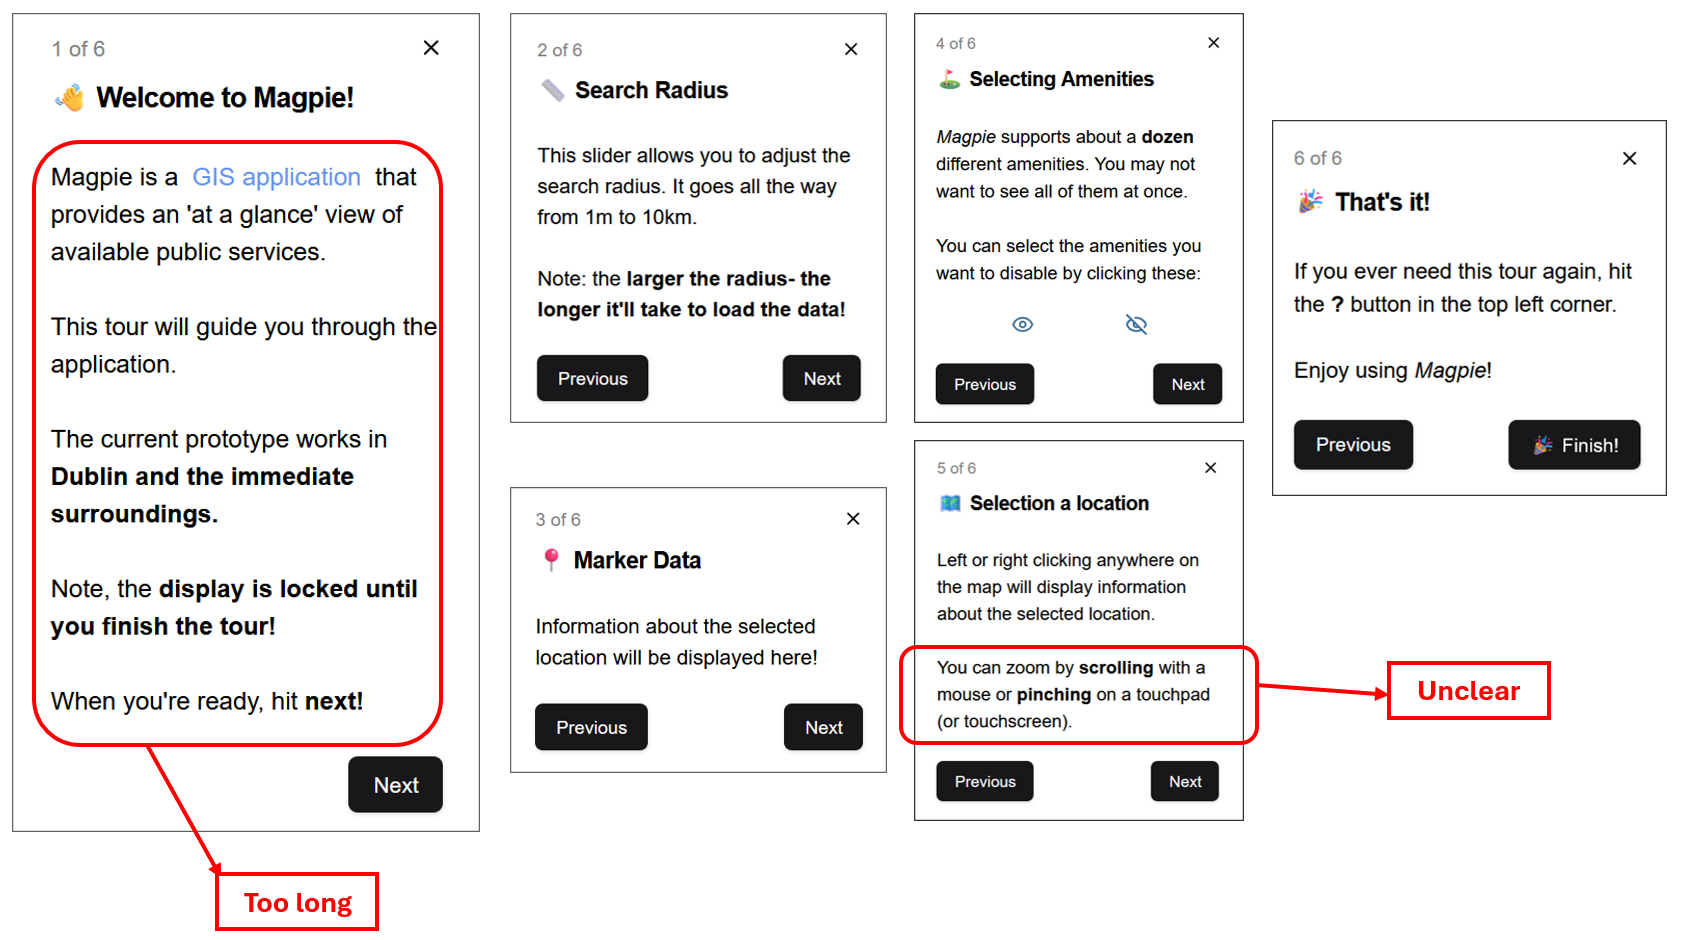
\includegraphics[width=0.9\textwidth]{images/onboarding-text-v1.png}
    \caption{V.0.1 Magpie Onboarding Steps}
\end{figure}

\newpage
\noindent\textbf{Map: }
Going back to the zooming feature Damian Gordon struggled with, adding zoom in and zoom out buttons directly on the map would offer an alternative to those not able to use the mouse for the action, further improving Magpie's accessibility.\\In addition, the profile and onboarding icons blended into the map which made it difficult for Damian Gordon to go back to the onboarding or log out as shown in the figure below.
%figure for the old icons for profile and onboarding
\begin{figure}[h!]
    \centering
    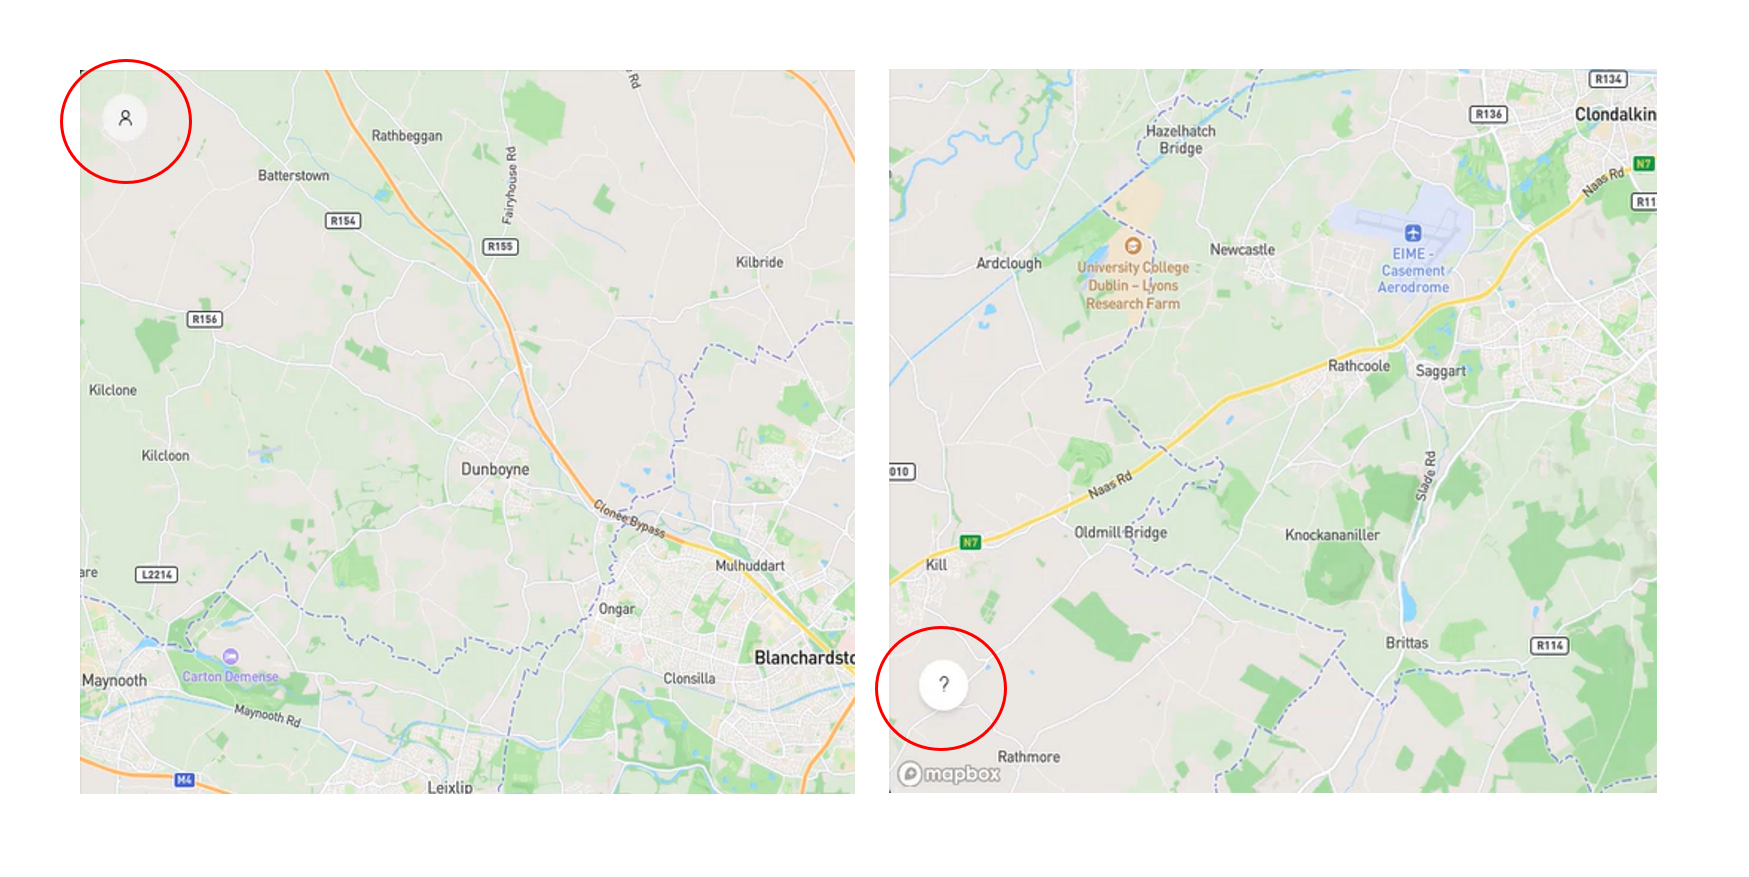
\includegraphics[width=0.8\textwidth]{images/old-icons-map.png}
    \caption{V.0.1 Magpie Profile \& Onboarding icons}
\end{figure}

\noindent Lastly, his survey responses confirmed that Magpie adheres to the WCAG guidelines detailed above as well as fulfils the major goal of ease of use. The survey covered 3 major sections: UI components, UI Design \& Language and UI interaction.\\

\noindent\textbf{UI Components} evaluate the position, quantity and accessibility of control elements such as the navigation buttons, the map controls, the dashboard toggles, etc\ldots Damian Gordon rated this section a \underline{4.75 out of 5}, the placement of control elements loosing one point because some of them were nested and therefore hard to notice or navigate to, like the profile and tutorial icons on the map mentioned above.
%figure for UI component survey response Damian
\begin{figure}[h!]
    \centering
    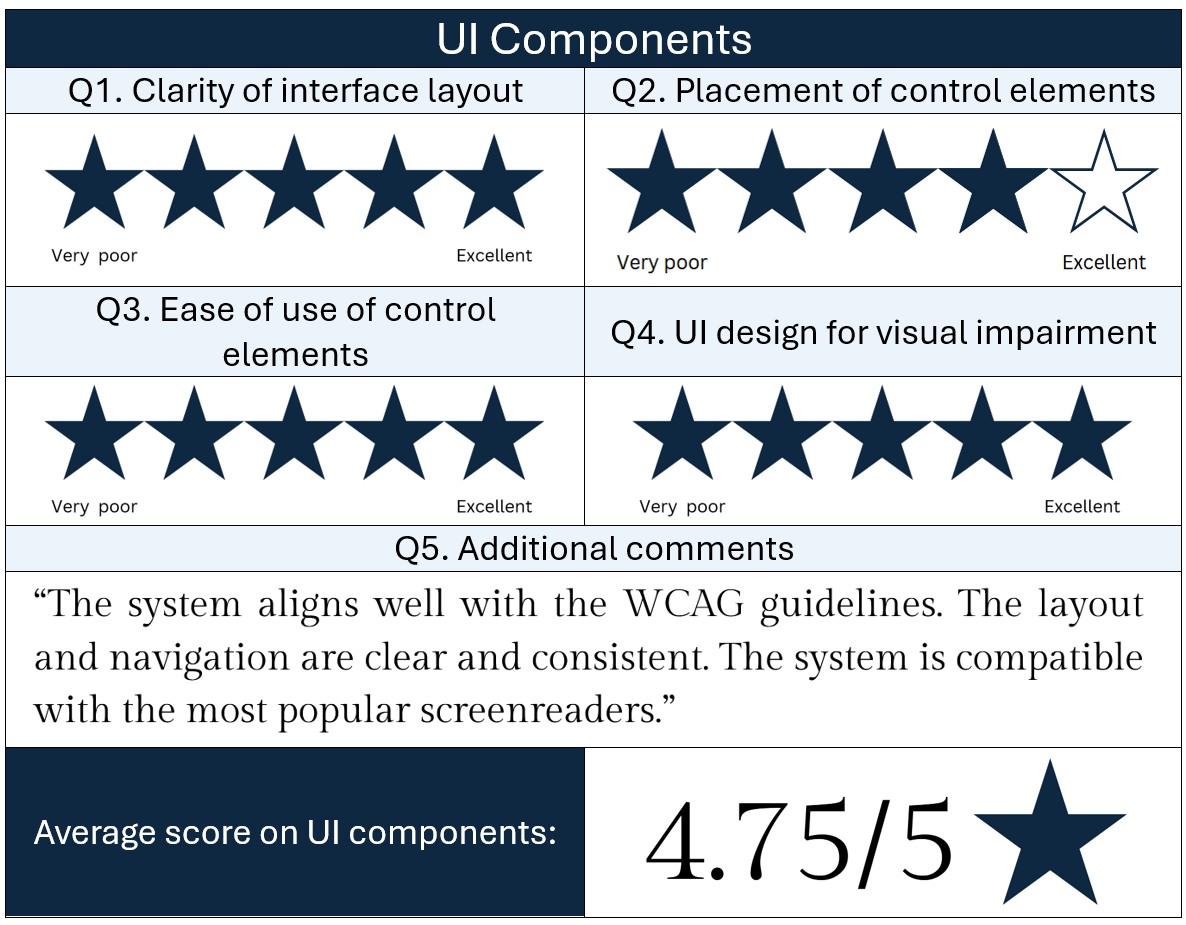
\includegraphics[width=0.6\textwidth]{images/accessb-survey-components.png}
    \caption{Accessibility review \- UI Components Score}
\end{figure}

\newpage
\noindent\textbf{UI Design \& Language} covers the style of UI components as well as the textual language used on the interface. Damian Gordon rated this aspect of Magpie at \underline{5 out of 5}, noting that there is a clear and effective use of language and icons which both are easily recognizable and clear.
%figure for UI design survey response Damian
\begin{figure}[h!]
    \centering
    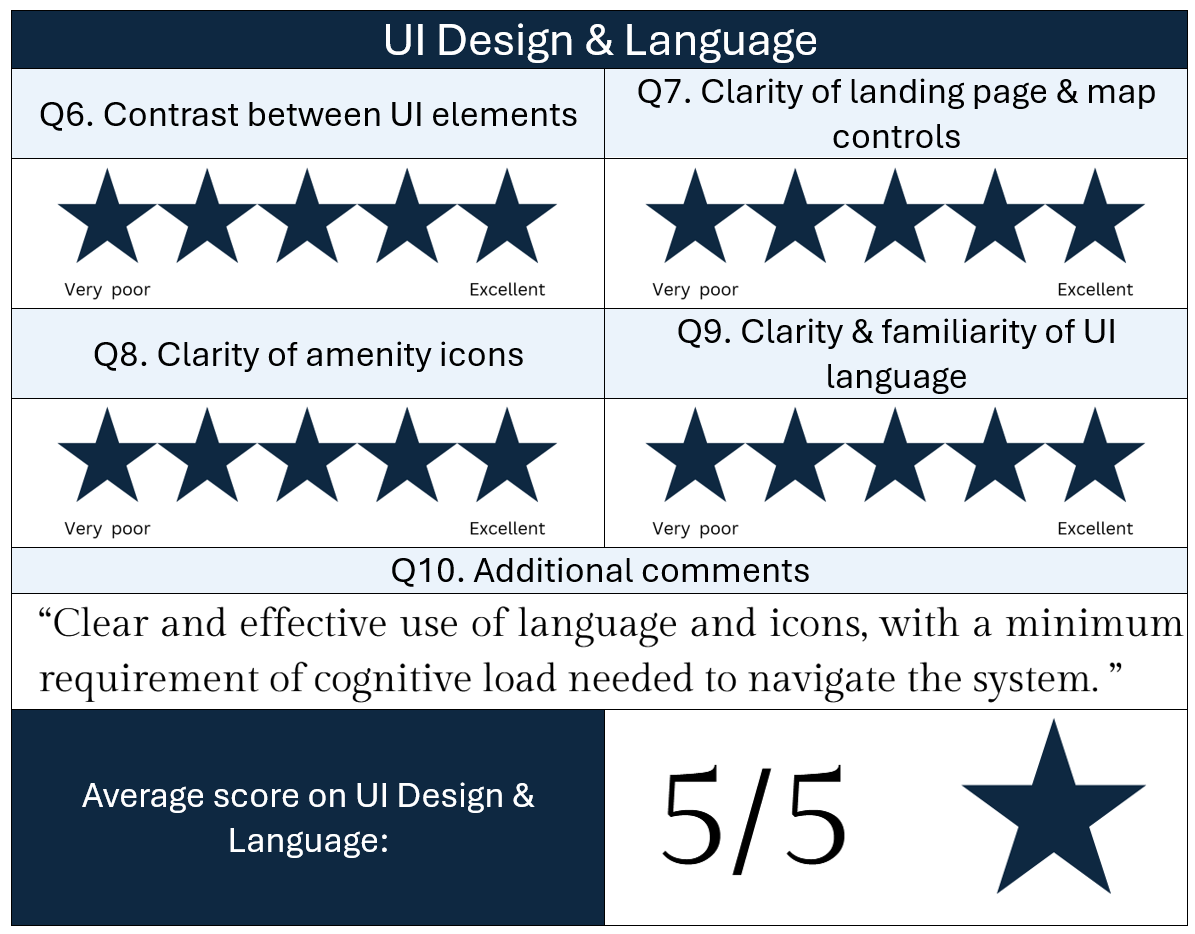
\includegraphics[width=0.6\textwidth]{images/accessb-survey-design.png}
    \caption{Accessibility review \- UI Design \& Language Score}
\end{figure}

\noindent The last section, \textbf{UI Interaction} covers the range of interaction possible with the Magpie UI using different hardware and software tools. Damian Gordon also rated this section a \underline{5 out of 5}, citing good compatibility with industry standard screen readers and ease of navigation with both keyboard and mouse.\\
%figure for UI interaction survey response Damian
\begin{figure}[h!]
    \centering
    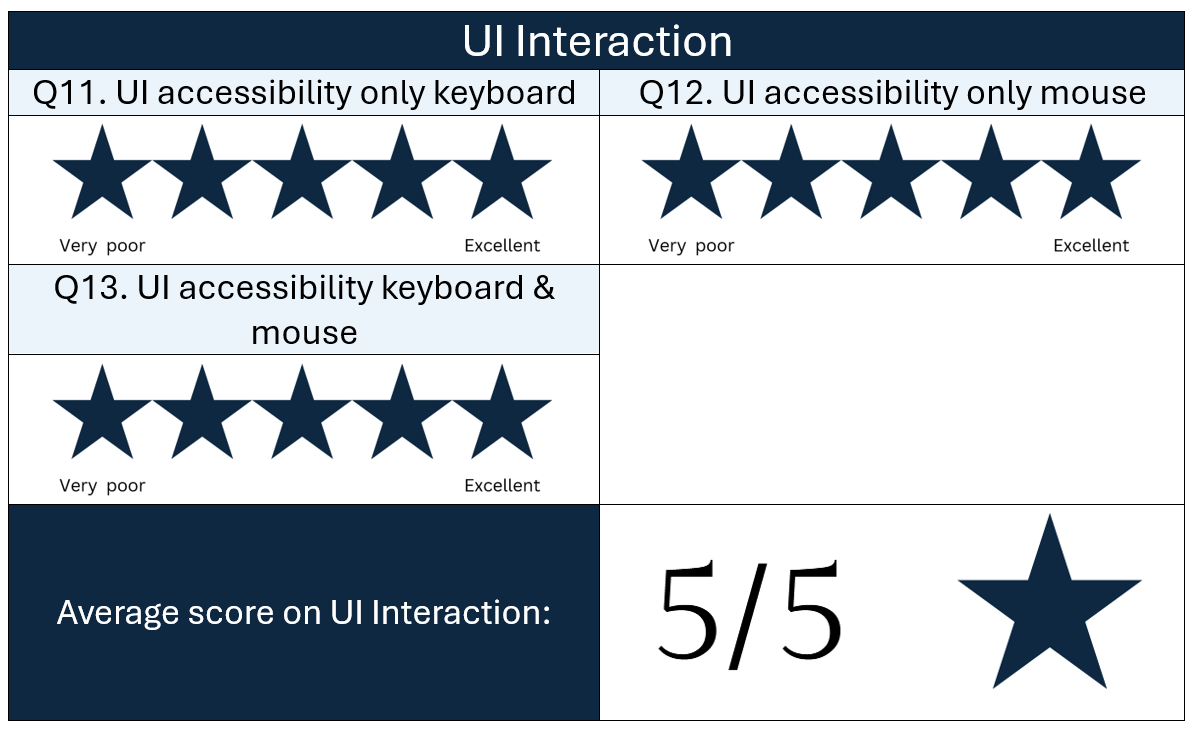
\includegraphics[width=0.6\textwidth]{images/accessb-survey-interaction.png}
    \caption{Accessibility review \- UI Interaction Score}
\end{figure}

\newpage
\noindent\textbf{Overall}, Magpie scores a \underline{4.92 out of 5} score in accessibility, with perfect scores in both UI design, language and interaction. Points to improve relate to increasing accessibility by reducing the number of nested elements, and making adjustments to the tutorial as per vocal recommendation during the testing session.
%figure for overall score survey response Damian
\begin{figure}[h!]
    \centering
    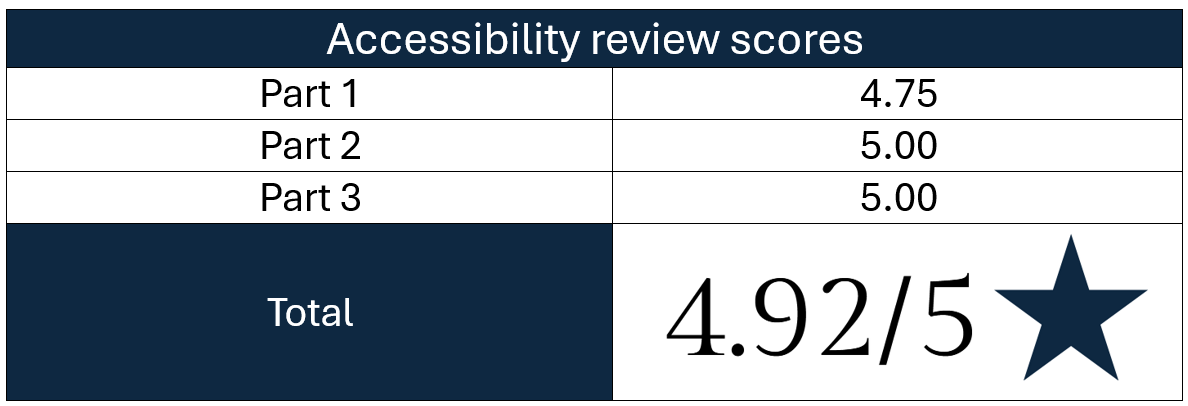
\includegraphics[width=0.8\textwidth]{images/accessb-survey-summary.png}
    \caption{Accessibility review \- Overall Score}
\end{figure}
